\documentclass[10pt,a4paper]{article}
\usepackage[margin=1in]{geometry}

\usepackage{polski}
\usepackage[utf8]{inputenc}

\usepackage{amsfonts}
\usepackage{amsthm}
\usepackage{enumerate}
\usepackage{graphicx}
\usepackage{indentfirst}
\usepackage{hyperref}

\usepackage{pgfplots}
\pgfplotsset{width=10cm,compat=1.9}
\usepgfplotslibrary{external}
\tikzexternalize 

\theoremstyle{definition}
\newtheorem{zad}{Zadanie}
\theoremstyle{definition}
\newtheorem{odp}{Zadanie}
\theoremstyle{definition}
\newtheorem{defi}{Definicja}

\newcommand{\NN}{\mathbb{N}}
\newcommand{\RR}{\mathbb{R}}
\newcommand{\QQ}{\mathbb{Q}}
\newcommand{\ZZ}{\mathbb{Z}}

\author{Łukasz Bratos}
\title{Sprawozdanie\\
    AiSD lista 4}
\date{maj 2019}

\begin{document}
\maketitle

\section{Wstęp}
    Celem listy było zaimplementowanie oraz przetestowanie następujących struktur danych:
    \begin{itemize}
        \item BST (drzewo poszukiwań binarnych)
        \item RBT (drzewo czerwono - czarne)
        \item Drzewo Splay (samoorganizujące drzewo binarne)
    \end{itemize}
    
    Struktury zostały zaimplementowane w języku Java.
\section{Drzewa}
    \subsection{BST}
        Drzewa poszukiwań binarnych, w skrócie BST (ang. Binary Search Trees), są strukturami na których można wykonywać różne operacje właściwe dla zbiorów dynamicznych, takie jak SEARCH, MINIMUM, MAXIMUM, PREDECESSOR, SUCCESSOR, INSERT oraz DELETE. Drzewo poszukiwań może więc być użyte zarówno jako słownik, jak i jako kolejka priorytetowa.
        
        Podstawowe operacje na drzewach poszukiwań binanrnych wymagają czasu proporcjonalnego do wysokości drzewa. W pełnym drzewie binarnym o $n$ węzłach takie operacje działają w najgorszym przypadku w czasie $O(\lg n)$. Jeśli jednak drzewo składa się z jednej gałęzi o długości $n$, to te same operacje wymagają w pesymistycznym przypadku czasu $O(n)$.
        
        Klucze są przechowywane w drzewie BST w taki sposób, aby spełniona była własność drzewa BST:
        \begin{defi}
            Niech $x$ będzie węzłem drzewa BST. Jeśli $y$ jest węzłem znajdującym się w lewym poddrzewie węzła $x$, to $y.key \leq x.key$. Jeśli $y$ jest węzłem znajdującym się w prawym poddrzewie węzła $x$, to $x.key \leq y.key$.
        \end{defi}
        
        \begin{figure}[h]
        	\centering
        	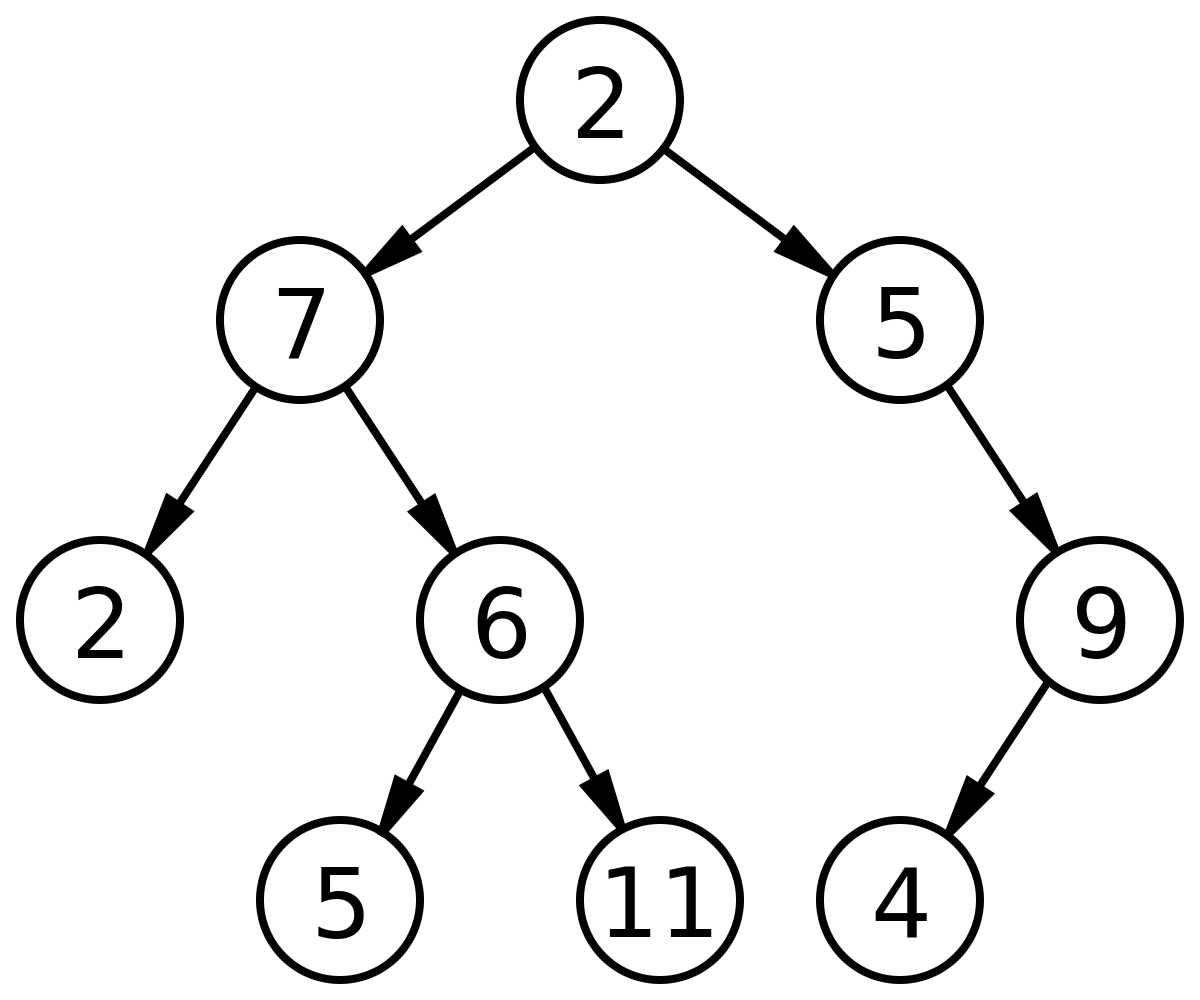
\includegraphics[scale=0.25]{images/bst}
        	\caption{Przykładowe drzewo poszukiwań binarnych}
        	\label{fig:bst}
       	\end{figure}
        
    \subsection{RBT}
        Drzewo czerwono - czarne jest drzewem poszukiwań binarnych, w którym na każdy węzeł przypada jeden dodatkowy bit informacji: jego kolor, który może być albo czerwony (RED), albo czarny (BLACK). Przez narzucenie odpowiednich warunków na możliwe ciągi kolorów węzłów leżących na dowolnej ścieżce biegnącej od korzenia do liścia drzewa czerwono - czarnego gwarantujemy, że każda ścieżka jest co najwyżej dwa razy dłuższa niż dowolna inna, dzięki czemu drzewo jest w przybliżeniu zrównoważone.
        
        Drzewo BST jest drzewem czerwono - czarnym, jeśli ma następujące własności czerwono - czarne:
        \begin{enumerate}
            \item każdy węzeł jest albo czerwony, albo czarny;
            \item korzeń jest czarny;
            \item każdy liść (NIL) jest czarny;
            \item jeśli węzeł jest czerwony, to obaj jego synowie są czarni;
            \item każda prosta ścieżka z ustalonego węzła do liścia ma tyle samo czarnych węzłów.
        \end{enumerate}
        
        \begin{figure}[h]
        	\centering
        	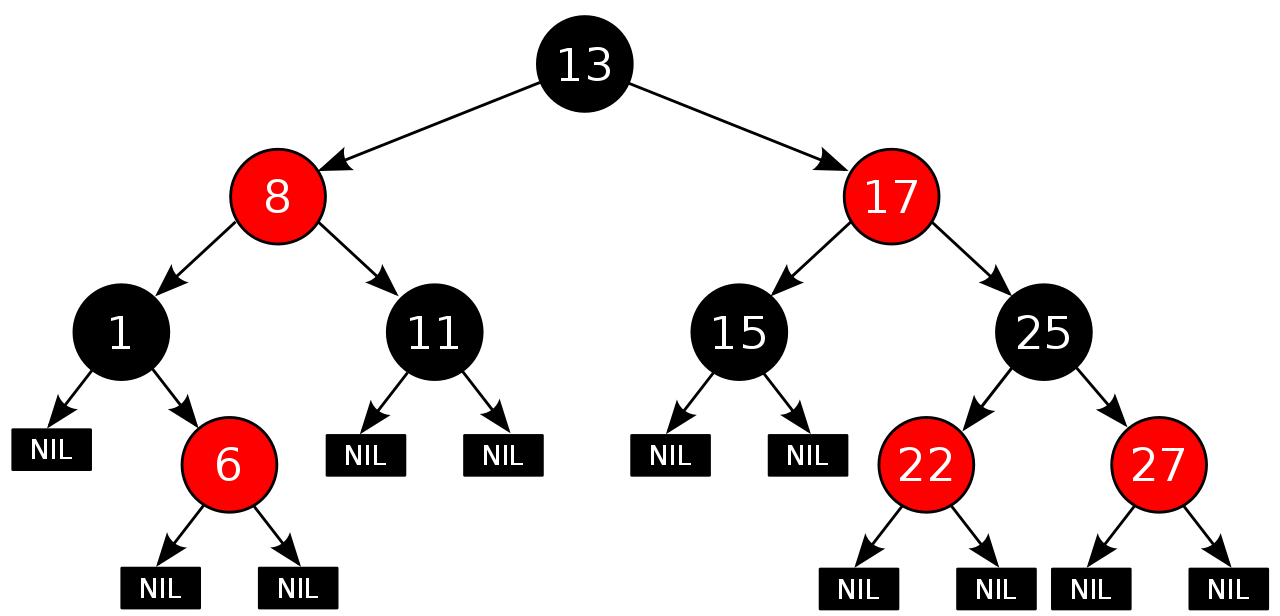
\includegraphics[scale=0.25]{images/rbt}
        	\caption{Przykładowe drzewo czerwono - czarne}
        	\label{fig:rbt}
       	\end{figure}
        
    \subsection{Splay}
        Drzewo splay to struktura danych w formie samodostosowującego się drzewa poszukiwań binarnych. Wykonywanie podstawowych operacji na drzewie splay wiąże się z wykonaniem procedury $Splay(T, x)$, która powoduje taką zmianę struktury drzewa $T$, że węzeł $x$ zostaje umieszczony w korzeniu przy zachowaniu porządku charakterystycznego dla drzewa BST.
        
        W porównaniu do innych drzew BST, drzewa splay zmieniają swoją strukturę również podczas wyszukiwana kluczy (a nie tylko dodawania lub usuwania), przesuwając znaleziony węzeł w kierunku korzenia, dzięki temu często wyszukiwane węzły stają się szybsze do znalezienia. Z tego powodu drzewa splay bywają wykorzystywane w systemach typu cache. Drzewa splay nie są samorównoważące, ponieważ ich wysokość nie jest ograniczona przez $O(\lg n)$ – można np. tak wykonać operacje, że drzewo zdegeneruje się do listy. 
\section{Testy}
    \subsection{Metodologia}
        Testy polegały na wczytaniu wszystkich słów w pliku, wyszukaniu ich, a następnie ich usunięciu.
        Dla każdego drzewa w każdym teście mierzone były czas działania, liczba porównań oraz liczba modyfikacji węzłów dla operacji \textit{insert, search, delete}. Testy był wykonywane 100 razy dla każdego pliku. Wynik to średnia arytmetyczna ze wszystkich 100 testów.
        
        Testy były przeprowadzone na następujących plikach:
        \begin{itemize}
            \item lotr.txt - plik z powtórzeniami
            \item aspell.txt - ciąg znaków w porządku leksykograficznym
            \item KJB.txt - duży plik z powtórzeniami
            \item permutation.txt - dla każdego testu losowa permutacja pliku lotr.txt
        \end{itemize}
    \subsection{Wyniki}
        \begin{table}[h]
            \centering
            \caption{Wyniki dla pliku lotr.txt}
            \label{tab:lotr}
            \begin{tabular}{|c|c|c|c|c|} \hline
            		 & Operacja & BST & RBT & Splay \\
            		\hline
            		Czas [s] & Insert & 5,793 & 0,105 & 0,108 \\
            		
            		& Search & 0,085 & 0,0522 & 0,078 \\
            	
            		& Delete & 0,069 & 0,088 & 0,140 \\
            		\hline
            		Porównania & Insert & 317 576 165 & 10 880 514 & 28 878 615 \\
            		& Search & 12 573 838 & 5 575 015 & 20 186 563 \\
            		& Delete & 9 509 763 & 9 794 607 & 26 171 327 \\
            		\hline
            		Modyfikacje & Insert & 3 379 275 & 3 193 751 & 14 580 045 \\
            		& Search & 0 & 0 & 9 162 265 \\
            		& Delete & 967 705 & 2 772 111 & 10 115 982 \\
            		\hline 
            \end{tabular}
            \end{table}
            
            \begin{table}[h]
            \centering
            \caption{Wyniki dla pliku aspell.txt}
            \label{tab:aspell}
            \begin{tabular}{|c|c|c|c|c|} \hline
            		 & Operacja & BST & RBT & Splay \\
            		\hline
            		Czas [s] & Insert & 179,241 & 0,056 & 0,035 \\
            		
            		& Search & 51,943 & 0,055 & 0,074 \\
            	
            		& Delete & 0,039 & 0,051 & 0,06 \\
            		\hline
            		Porównania & Insert & 15 869 952 574 & 8 918 531 & 1 637 666 \\
            		& Search & 233 804 613 925 & 6 059 926 & 6 135 476 \\
            		& Delete & 755 850 & 7 199 810 & 5 615 808 \\
            		\hline
            		Modyfikacje & Insert & 251 949 & 2 078 210 & 755 845 \\
            		& Search & 0 & 0 & 2 492 963 \\
            		& Delete & 125 974 & 1 007 622 & 2 105 212 \\
            		\hline 
            \end{tabular}
            \end{table}
            
            \begin{table}[h]
            \centering
            \caption{Wyniki dla pliku KJB.txt}
            \label{tab:kjb}
            \begin{tabular}{|c|c|c|c|c|} \hline
            		 & Operacja & BST & RBT & Splay \\
            		\hline
            		Czas [s] & Insert & 268,383 & 0,560 & 0,486 \\
            		
            		& Search & 0,387 & 0,242 & 0,326 \\
            	
            		& Delete & 0,322 & 0,355 & 3,922 \\
            		\hline
            		Porównania & Insert & 12 628 705 658 & 582 023 342 & 116 327 704 \\
            		& Search & 51 918 408 & 24 224 577 & 710 933 137 \\
            		& Delete & 386 339 751 & 45 245 189 & 531 003 874 \\
            		\hline
            		Modyfikacje & Insert & 1 704 605 & 145 633 628 & 58 495 699 \\
            		& Search & 0 & 0 & 31 892 857 \\
            		& Delete & 4 343 619 & 12 718 738 & 36 817 366 \\
            		\hline 
            \end{tabular}
            \end{table}
            
            \begin{table}[h]
            \centering
            \caption{Wyniki dla losowych permutacji pliku lotr.txt}
            \label{tab:permutations}
            \begin{tabular}{|c|c|c|c|c|} \hline
            		 & Operacja & BST & RBT & Splay \\
            		\hline
            		Czas [s] & Insert & 4,902 & 0,106 & 0,115 \\
            		
            		& Search & 0,058 & 0,046 & 0,074 \\
            	
            		& Delete & 0,058 & 0,078 & 0,132 \\
            		\hline
            		Porównania & Insert & 312 359 747 & 10 780 871 & 29 772 722 \\
            		& Search & 7 815 644 & 5 603 440 & 21 602 571 \\
            		& Delete & 8 292 971 & 9 787 674 & 27 802 732 \\
            		\hline
            		Modyfikacje & Insert & 378 066 & 3 148 830 & 15 052 097 \\
            		& Search & 0 & 0 & 9 836 913 \\
            		& Delete & 991 138 & 2 752 475 & 10 794 134 \\
            		\hline 
            \end{tabular}
            \end{table}
            
            % \begin{table}[h]
            % \centering
            % \caption{Wyniki dla losowych permutacji pliku lotr.txt}
            % \label{tab:lotr}
            % \begin{tabular}{|c|c|c|c|c|} \hline
            % 		 & Operacja & BST & RBT & Splay \\
            % 		\hline
            % 		Czas [s] & Insert &  &  &  \\
            		
            % 		& Search &  &  &  \\
            	
            % 		& Delete &  &  &  \\
            % 		\hline
            % 		Porównania & Insert &  &  &  \\
            % 		& Search &  &  &  \\
            % 		& Delete &  &  &  \\
            % 		\hline
            % 		Modyfikacje & Insert &  &  &  \\
            % 		& Search &  &  &  \\
            % 		& Delete &  &  &  \\
            % 		\hline 
            % \end{tabular}
            % \end{table}
            
\section{Wnioski}
    Na podstawie testów możemy wywnioskować jak zachowują się poszczególne struktury oraz skonfrontować to z teorią. Pierwszą obserwacją jest to jak operacja insert w BST odstaje od pozostałych struktur. Może to być spowodowane brakiem jakiejkolwiek samoorganizacji, przez co złożoność czasowa, która jest proporcjonalna do wysokości drzewa, w pesymistycznym przypadku jest liniowa. Widać to dobrze w przypadku posortowanego pliku gdzie liczba porównań dla operacji insert oraz search gwałtownie wzrasta.
    
    RBT wypada bardzo dobrze w każdych testach niezależnie od pliku.
    
    Samoorganizacja drzewa splay znacząco przyspiesza operację insert w stosunku do BST. Operacja search w przypadku gdy dane są posortowane również przyspiesza. To wszystko niestety odbywa się kosztem operacji delete, która w każdym z testowanych przez nas przypadków działa wolniej niż w BST.
    
    
    \subsection{Preferowane rodzaje danych}
        \subsubsection{BST}
            BST najgorzej współgra z danymi posortowanymi - drzewo jest wtedy degenerowane do listy. Aby temu zapobiec dane powinny być podawane w takiej kolejności aby wynikowe drzewo było jak najbardziej zbalansowane. Pozwoli to uzyskać rzeczywistą złożoność logarytmiczną. Dane takie można uzyskać sczytując je wiersz po wierszu z drzewa RBT.
        \subsubsection{RBT}
            Z testów wynika, że RBT spisuje się świetnie dla każdych danych. Najmniej porównań oraz modyfikacji wykonuje jednak na danych posortowanych.
        \subsubsection{Splay}
            Ze względu na specyfikę funkcji splay, która jest wywoływana po każdej operacji i przesuwa dane o które pytaliśmy w górę drzewa, możemy spodziewać się drzewo splay najlepiej będzie się zachowywać w przypadku częstego pytania o te same dane.
\section{Bibliografia}
    \begin{enumerate}
        \item \textit{Introduction to Algorithms by Thomas H. Cormen, Charles E. Leiserson, Ronald L. Rivest, Clifford Stein}
        \item \href{https://pl.wikipedia.org/wiki/Drzewo_splay}{\textit{pl.wikipedia.org/wiki/Drzewo\_splay}}
    \end{enumerate}{}
    
\end{document}